\runningheader{Computer Science Principles}{AP Practice Exam (Coding / Programming)}{Page \thepage\ of \numpages}

\begingradingrange{cspcoding}

\question[5]
What will the following program display?\footnote{AP CSP pseudocode uses 1-based indexing for lists, so the first element is at index 1.}
\begin{lstlisting}[style=pseudo]
list <- [11, 35, 6, 0]
DISPLAY(mystery(list))

PROCEDURE mystery(list)
{
  sum <- 0
  FOR EACH item IN list
  {
    sum <- sum + item
  }
  RETURN sum / LENGTH(list)
}
\end{lstlisting}
\begin{choices}
  \choice 0
  \choice 4
  \choice 13
  \CorrectChoice 35
\end{choices}
\begin{solution}
  \((11+35+6+0)/4 = 52/4 = 13\).
\end{solution}

\question[5]
What will the following program display?
\begin{lstlisting}[style=pseudo]
list <- [11, 35, 6]
DISPLAY(mystery(list))

PROCEDURE mystery(list)
{
  max <- list[1]
  FOR EACH item IN list
  {
    IF (item > max)
    {
      max <- item
    }
  }
  RETURN max
}
\end{lstlisting}
\begin{choices}
  \choice 0
  \choice 12
  \choice 16
  \CorrectChoice 35
\end{choices}
\begin{solution}
  The maximum value in the list is 35.
\end{solution}

\newpage 

\question[5]
What will the following program display?
\begin{lstlisting}[style=pseudo]
list1 <- [1, 1, 35, 6, 76, 4, 98]
list2 <- []

FOR EACH item IN list1
{
  IF (item MOD 2 = 0)
  {
    APPEND(list2, item)
  }
}

DISPLAY(list2)
\end{lstlisting}
\begin{choices}
  \CorrectChoice \texttt{[6, 76, 4, 98]}
  \choice \texttt{[1, 1, 35]}
  \choice \texttt{[1, 1, 35, 6, 76, 4, 98]}
  \choice \texttt{[]}
\end{choices}
\begin{solution}
  The code filters even values into \texttt{list2}.
\end{solution}

\question[5]
What will the following program display?
\begin{lstlisting}[style=pseudo]
list <- [11, 35, 6, 2]
DISPLAY(mystery(list))

PROCEDURE mystery(list)
{
  sum <- list[1]
  count <- 1
  n <- LENGTH(list)
  REPEAT (n - 2) TIMES
  {
    sum <- sum + list[count]
    count <- count + 1
  }
  RETURN (sum / count)
}
\end{lstlisting}
\begin{choices}
  \choice 0
  \choice 13
  \choice 16
  \CorrectChoice 19
\end{choices}
\begin{solution}
  \texttt{n = 4}, so the loop repeats \(n-2=2\) times. Starting with \texttt{sum = 11} and \texttt{count = 1}, the loop adds \texttt{list[1]} and \texttt{list[2]}, giving \texttt{sum = 57} and \texttt{count = 3}. The program returns \(57/3 = 19\).
\end{solution}

\newpage

\question[5]
What will the following program display?
\begin{lstlisting}[style=pseudo]
list1 <- [1, 1, 35, 6, 76, 4, 98]
list2 <- []

FOR EACH item IN list1
{
  IF (item MOD 2 = 1)
  {
    APPEND(list2, item)
  }
}

DISPLAY(list2)
\end{lstlisting}
\begin{choices}
  \choice \texttt{[6, 76, 4, 98]}
  \CorrectChoice \texttt{[1, 1, 35]}
  \choice \texttt{[1, 1, 35, 6, 76, 4, 98]}
  \choice \texttt{[]}
\end{choices}
\begin{solution}
  The code keeps odd values only.
\end{solution}

\question[5]
What will the following program display?
\begin{lstlisting}[style=pseudo]
list1 <- [1, 1, 35, 6, 76, 4, 98]
list2 <- []

FOR EACH item IN list1
{
  IF (item MOD 2 = 0 AND item MOD 2 = 1)
  {
    APPEND(list2, item)
  }
}

DISPLAY(list2)
\end{lstlisting}
\begin{choices}
  \choice \texttt{[0]}
  \choice \texttt{[-11]}
  \choice \texttt{[-35]}
  \CorrectChoice \texttt{[]}
\end{choices}
\begin{solution}
  No integer can be both even and odd at the same time.
\end{solution}

\newpage 

\question[5]
What will the following program display?
\begin{lstlisting}[style=pseudo]
list1 <- [1, 1, 35, 6, 76, 4, 98]
list2 <- []

FOR EACH item IN list1
{
  IF (item MOD 2 = 0 OR item MOD 2 = 1)
  {
    APPEND(list2, item)
  }
}

DISPLAY(list2)
\end{lstlisting}
\begin{choices}
  \choice \texttt{[6, 76, 4, 98]}
  \choice \texttt{[1, 1, 35]}
  \CorrectChoice \texttt{[1, 1, 35, 6, 76, 4, 98]}
  \choice \texttt{[]}
\end{choices}
\begin{solution}
  Every listed integer is either even or odd, so all values are appended.
\end{solution}

\question[5]
What will the following program display?
\begin{lstlisting}[style=pseudo]
list1 <- [41, 1, 35, 6, 76, 4, 98]
max <- list1[1]

FOR EACH item IN list1
{
  IF (item > max)
  {
    max <- item
  }
}

DISPLAY(max)
\end{lstlisting}
\begin{choices}
  \choice 1
  \CorrectChoice 98
  \choice 0
  \choice 76
\end{choices}
\begin{solution}
  The running maximum ends at 98.
\end{solution}

\newpage 

\question[5]
What will the following program display?
\begin{lstlisting}[style=pseudo]
list1 <- [1, 1, 35, 6, 76, 4, 98]
max <- 0
FOR EACH item IN list1
{
  IF (item > max)
  {
    max <- item
  }
}

DISPLAY(max)
\end{lstlisting}
\begin{choices}
  \choice 0
  \choice 98
  \choice 1
  \CorrectChoice -98
\end{choices}
\begin{solution}
  The running maximum ends at -98.
\end{solution}

\newpage

\question[5]
The following question uses a robot in a grid of squares. The robot is represented as a triangle, which is initially in the top-left square of the grid and facing toward the top of the grid.
\begin{center}
  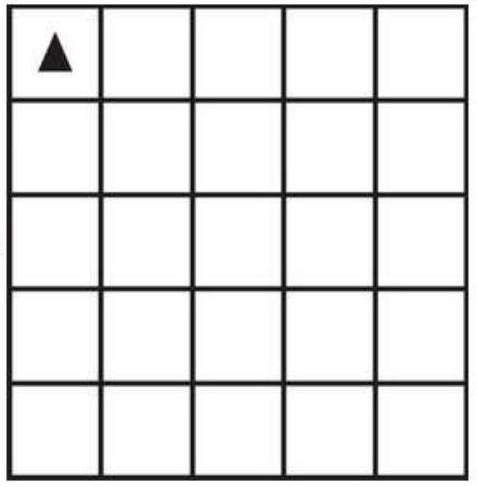
\includegraphics[width=0.26\linewidth]{cs-p/images/28f8d221-10b3-4a50-9845-f8cdfb9b0a46-20_493_510_1903_34}
\end{center}
Code for the procedure Mystery is shown here. Assume that the parameter \texttt{p} has been assigned a positive integer value (e.g., 1, 2, 3, \ldots).
\begin{lstlisting}[style=pseudo]
  PROCEDURE Mystery(p)
  {
    REPEAT p TIMES
    {
      ROTATE_RIGHT
      MOVE_FORWARD
      MOVE_FORWARD
    }
  }
\end{lstlisting}
Which of the following shows a possible result of calling the procedure?
\begin{center}
  \begin{minipage}[t]{0.24\linewidth}\centering
    \textbf{(A)}\\[0.5em]
    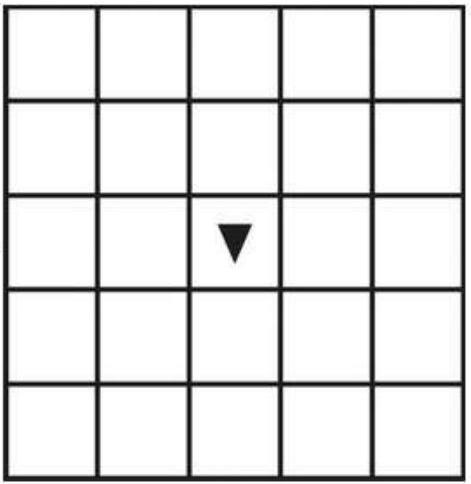
\includegraphics[width=\linewidth]{cs-p/images/28f8d221-10b3-4a50-9845-f8cdfb9b0a46-10_484_471_1394_120}
  \end{minipage}\hfill
  \begin{minipage}[t]{0.24\linewidth}\centering
    \textbf{(B)}\\[0.5em]
    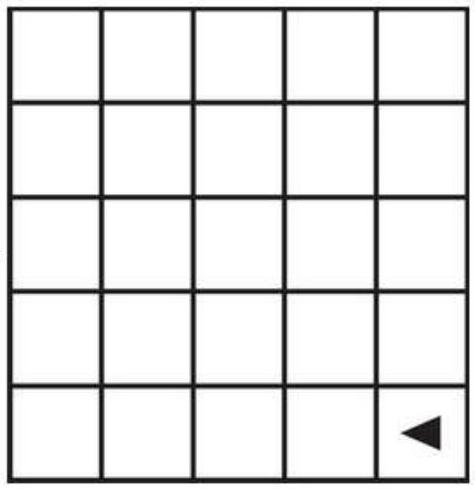
\includegraphics[width=\linewidth]{cs-p/images/28f8d221-10b3-4a50-9845-f8cdfb9b0a46-10_489_475_1886_116}
  \end{minipage}
  \begin{minipage}[t]{0.24\linewidth}\centering
    \textbf{(C)}\\[0.5em]
    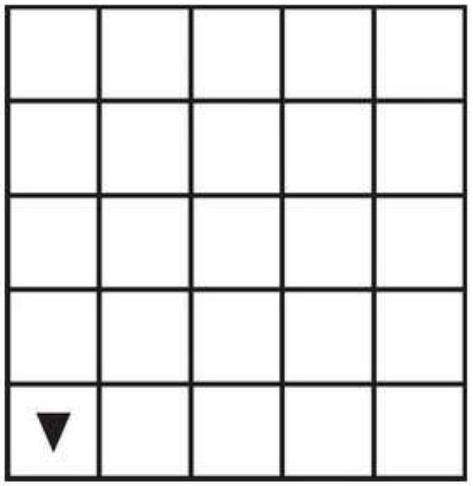
\includegraphics[width=\linewidth]{cs-p/images/28f8d221-10b3-4a50-9845-f8cdfb9b0a46-10_486_473_1394_711}
  \end{minipage}\hfill
  \begin{minipage}[t]{0.24\linewidth}\centering
    \textbf{(D)}\\[0.5em]
    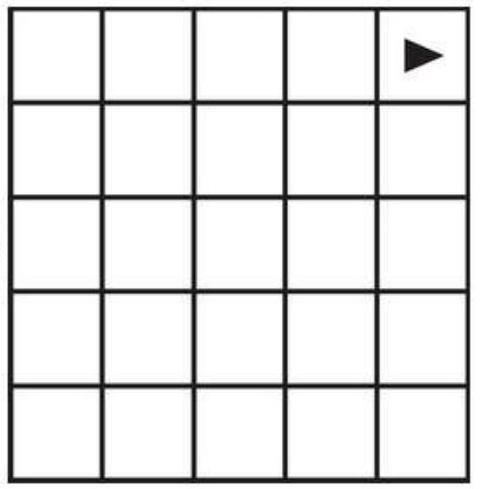
\includegraphics[width=\linewidth]{cs-p/images/28f8d221-10b3-4a50-9845-f8cdfb9b0a46-10_489_481_1886_708}
  \end{minipage}
\end{center}
\begin{choices}
  \choice (A)
  \choice (B)
  \choice (C)
  \choice (D)
\end{choices}
\begin{solution}
  Use the answer key associated with the source diagram set for this item.
\end{solution}

\newpage

\question[5]
The following question uses a robot in a grid of squares. The robot is represented as a triangle, which is initially in the top-left square of the grid and facing toward the top of the grid.
\begin{center}
  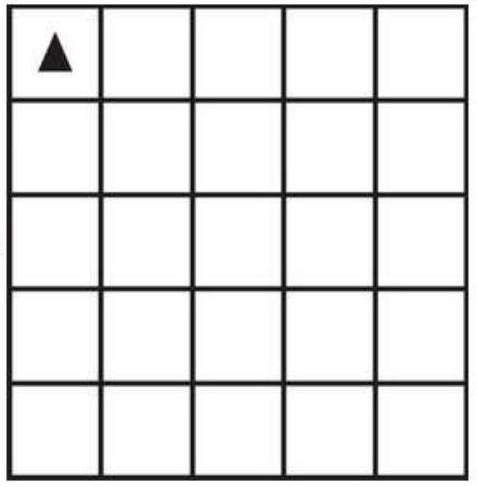
\includegraphics[width=0.26\linewidth]{cs-p/images/28f8d221-10b3-4a50-9845-f8cdfb9b0a46-20_493_510_1903_34}
\end{center}
Code for the procedure Mystery is shown below. Assume that the parameter \texttt{p} has been assigned a positive integer value (e.g., 1, 2, 3, \ldots).
\begin{lstlisting}[style=pseudo]
  PROCEDURE Mystery(p)
  {
    REPEAT p TIMES
    {
      ROTATE_LEFT
      MOVE_FORWARD
      ROTATE_RIGHT
    }
  }
  \end{lstlisting}
Which of the following shows the result of calling the procedure when \(p=4\)?
\begin{center}
  \begin{minipage}[t]{0.24\linewidth}\centering
    \textbf{(A)}\\[0.5em]
    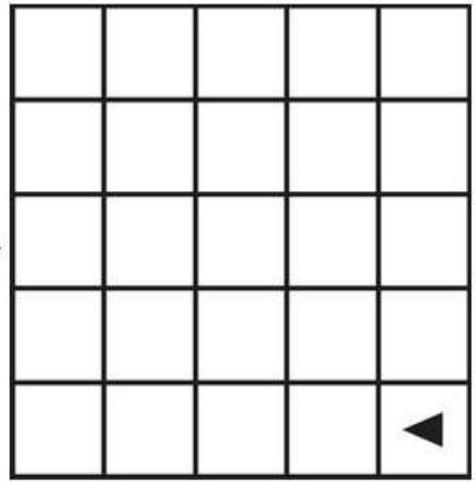
\includegraphics[width=\linewidth]{cs-p/images/28f8d221-10b3-4a50-9845-f8cdfb9b0a46-11_482_476_1587_214}
  \end{minipage}\hfill
  \begin{minipage}[t]{0.24\linewidth}\centering
    \textbf{(B)}\\[0.5em]
    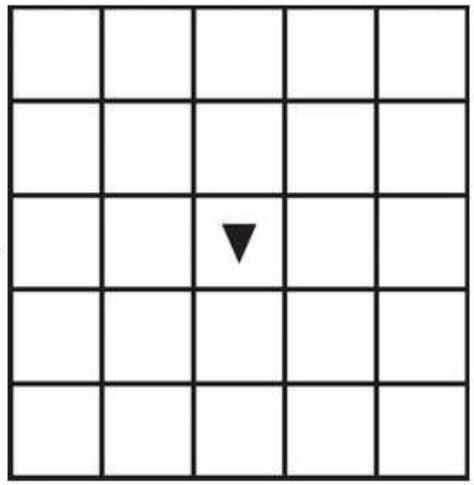
\includegraphics[width=\linewidth]{cs-p/images/28f8d221-10b3-4a50-9845-f8cdfb9b0a46-11_485_474_2079_216}
  \end{minipage}
  \begin{minipage}[t]{0.24\linewidth}\centering
    \textbf{(C)}\\[0.5em]
    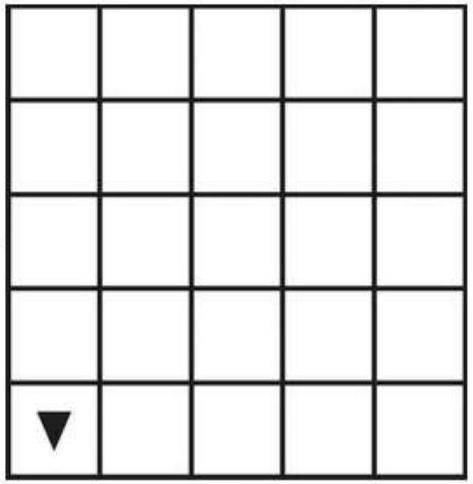
\includegraphics[width=\linewidth]{cs-p/images/28f8d221-10b3-4a50-9845-f8cdfb9b0a46-11_484_473_1585_812}
  \end{minipage}\hfill
  \begin{minipage}[t]{0.24\linewidth}\centering
    \textbf{(D)}\\[0.5em]
    Error (robot leaves the grid)
  \end{minipage}
\end{center}
\begin{choices}
  \choice (A)
  \choice (B)
  \choice (C)
  \choice (D)
\end{choices}
\begin{solution}
  Trace one full loop: left turn, move, and heading restoration.
\end{solution}


\newpage

\question[5]
The following question uses a robot in a grid of squares. The robot is represented as a triangle, which is initially in the top-left square of the grid and facing toward the top of the grid.
\begin{center}
  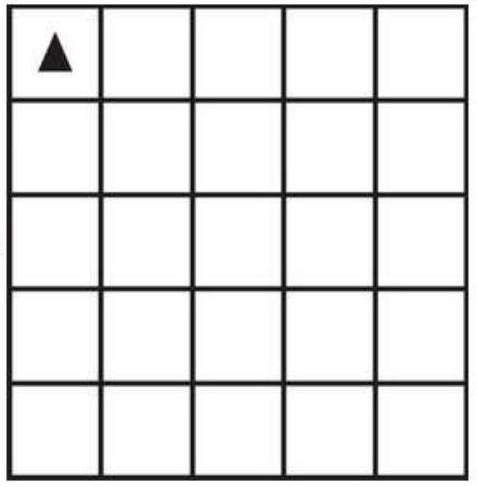
\includegraphics[width=0.26\linewidth]{cs-p/images/28f8d221-10b3-4a50-9845-f8cdfb9b0a46-20_493_510_1903_34}
\end{center}
Code for the procedure Mystery is shown below. Assume that the parameter \texttt{p} has been assigned a positive integer value (e.g., 1, 2, 3, \ldots).
\begin{lstlisting}[style=pseudo]
  PROCEDURE Mystery(p)
  {
    REPEAT p TIMES
    {
      ROTATE_RIGHT
      MOVE_FORWARD
      ROTATE_LEFT
    }
  }
\end{lstlisting}
Which of the following shows the result of calling the procedure when \(p=4\)?
\begin{center}
  \begin{minipage}[t]{0.24\linewidth}\centering
    \textbf{(A)}\\[0.5em]
    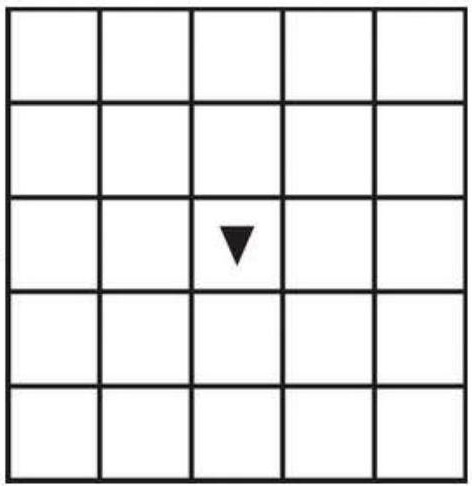
\includegraphics[width=\linewidth]{cs-p/images/28f8d221-10b3-4a50-9845-f8cdfb9b0a46-12_486_501_1366_47}
  \end{minipage}\hfill
  \begin{minipage}[t]{0.24\linewidth}\centering
    \textbf{(B)}\\[0.5em]
    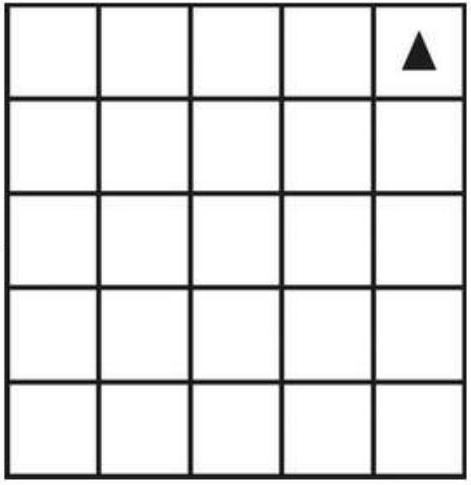
\includegraphics[width=\linewidth]{cs-p/images/28f8d221-10b3-4a50-9845-f8cdfb9b0a46-12_485_471_1864_77}
  \end{minipage}
  \begin{minipage}[t]{0.24\linewidth}\centering
    \textbf{(C)}\\[0.5em]
    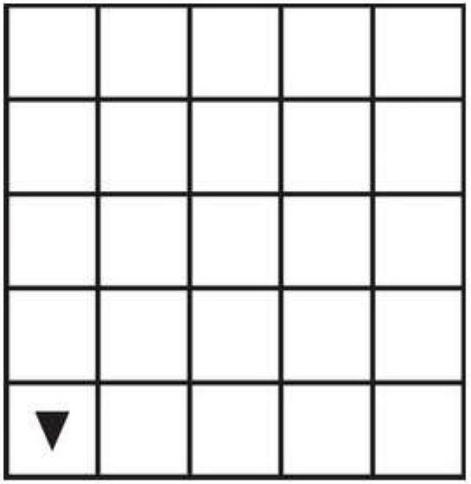
\includegraphics[width=\linewidth]{cs-p/images/28f8d221-10b3-4a50-9845-f8cdfb9b0a46-12_484_471_1366_653}
  \end{minipage}\hfill
  \begin{minipage}[t]{0.24\linewidth}\centering
    \textbf{(D)}\\[0.5em]
    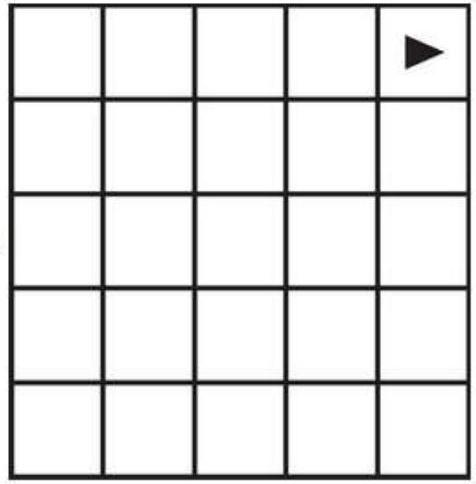
\includegraphics[width=\linewidth]{cs-p/images/28f8d221-10b3-4a50-9845-f8cdfb9b0a46-12_484_476_1860_648}
  \end{minipage}
\end{center}
\begin{choices}
  \choice (A)
  \choice (B)
  \choice (C)
  \choice (D)
\end{choices}
\begin{solution}
  The robot shifts right each cycle and restores orientation.
\end{solution}

\newpage

\question[5]
The program below is intended to find the highest non-negative number in a list.
\begin{lstlisting}[style=pseudo]
list <- [1, -2, 3, 0, -7]
result <- 0

FOR EACH item IN list
{
  IF (item < result)
  {
    result <- item
  }
}

DISPLAY(result)
\end{lstlisting}
Does the program work as intended?
\begin{choices}
  \choice Yes; it displays 1.
  \choice No; \texttt{result} starts at 0.
  \choice Yes; it displays 3.
  \CorrectChoice No; the conditional should be \texttt{item > result}.
\end{choices}
\begin{solution}
  The code as written searches downward, not upward.
\end{solution}

\question[5]
The following program is intended to find the lowest number in \texttt{list}.
\begin{lstlisting}[style=pseudo]
list <- [1, -2, 3, 10, -7]
result <- list[1]

FOR EACH item IN list
{
  IF (item < result)
  {
    result <- list[1]
  }
}

DISPLAY(result)
\end{lstlisting}
Does the program work as intended?
\begin{choices}
  \choice Yes; it displays -7.
  \CorrectChoice No; \texttt{result} is repeatedly reset to \texttt{list[1]}.
  \choice Yes; it displays 1.
  \choice No; runtime error.
\end{choices}
\begin{solution}
  Update should be \texttt{result <- item}, not \texttt{list[1]}.
\end{solution}

\newpage

\question[5]
The following program is intended to find the lowest number in \texttt{list}.
\begin{lstlisting}[style=pseudo]
list <- [1, 5, 9, 10]
result <- 0

FOR EACH item IN list
{
  IF (item < result)
  {
    result <- item
  }
}

DISPLAY(result)
\end{lstlisting}
Does the program work as intended?
\begin{choices}
  \choice Yes; it returns 10.
  \CorrectChoice No; it runs but returns a logical error of 0.
  \choice Yes; it returns 1.
  \choice No; runtime error.
\end{choices}
\begin{solution}
  With all-positive values, no item is \(< 0\), so \texttt{result} stays 0.
\end{solution}

\question[5]
The following program is intended to find the greatest number in \texttt{list}.
\begin{lstlisting}[style=pseudo]
list <- [-3, -5, -200, -1]
result <- list[1]

FOR EACH item IN list
{
  IF (item > result)
  {
    result <- item
  }
}

DISPLAY(result)
\end{lstlisting}
Does the program work as intended?
\begin{choices}
  \choice Yes; it returns -200.
  \choice No; \texttt{result} never changes and returns -3.
  \CorrectChoice Yes; it returns -1.
  \choice No; runtime error.
\end{choices}
\begin{solution}
  The largest value in the list is \(-1\).
\end{solution}

\newpage

\question[5]
The following question uses a robot in a grid of squares. The robot is represented as a triangle, which is initially in the top-left square of the grid and facing toward the top of the grid.
\begin{center}
  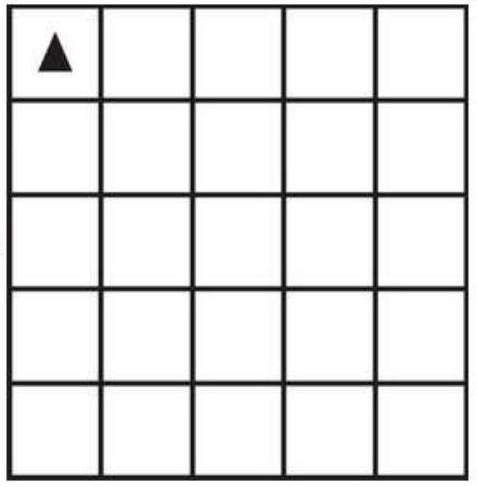
\includegraphics[width=0.26\linewidth]{cs-p/images/28f8d221-10b3-4a50-9845-f8cdfb9b0a46-20_493_510_1903_34}
\end{center}
Code for the procedure Mystery is shown below. Assume that the parameter \texttt{p} has been assigned a positive integer value (e.g., 1, 2, 3, \ldots).
\begin{lstlisting}[style=pseudo]
  PROCEDURE Mystery(p)
  {
    REPEAT p TIMES
    {
      ROTATE_LEFT
      MOVE_FORWARD
    }
  }
\end{lstlisting}
Which of the following shows the result of calling the procedure when \(p=6\)?
\begin{center}
  \begin{minipage}[t]{0.24\linewidth}\centering
    \textbf{(A)}\\[0.5em]
    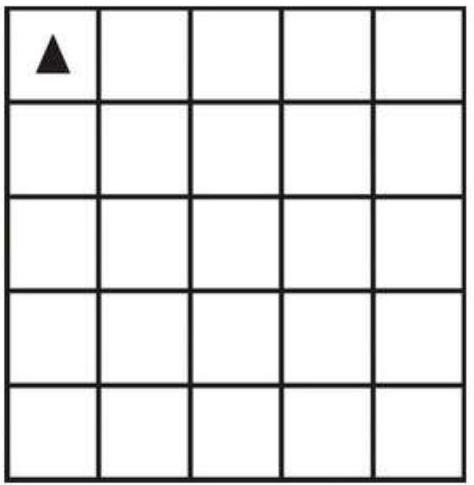
\includegraphics[width=\linewidth]{cs-p/images/28f8d221-10b3-4a50-9845-f8cdfb9b0a46-17_485_474_1370_70}
  \end{minipage}\hfill
  \begin{minipage}[t]{0.24\linewidth}\centering
    \textbf{(B)}\\[0.5em]
    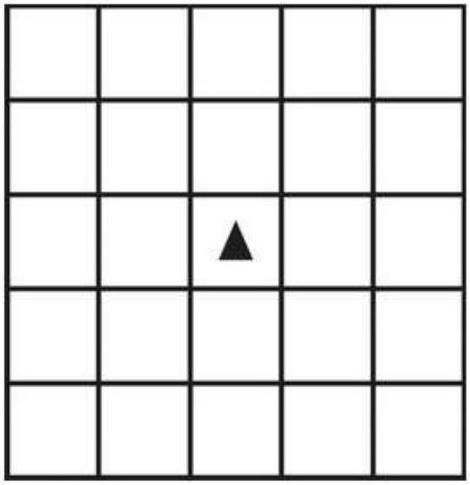
\includegraphics[width=\linewidth]{cs-p/images/28f8d221-10b3-4a50-9845-f8cdfb9b0a46-17_485_470_1866_70}
  \end{minipage}
  \begin{minipage}[t]{0.24\linewidth}\centering
    \textbf{(C)}\\[0.5em]
    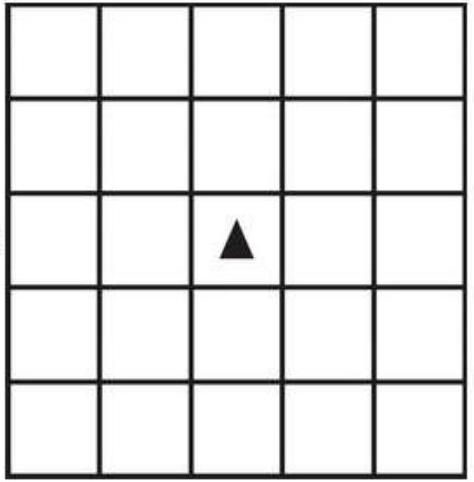
\includegraphics[width=\linewidth]{cs-p/images/28f8d221-10b3-4a50-9845-f8cdfb9b0a46-17_482_474_1370_663}
  \end{minipage}\hfill
  \begin{minipage}[t]{0.24\linewidth}\centering
    \textbf{(D)}\\[0.5em]
    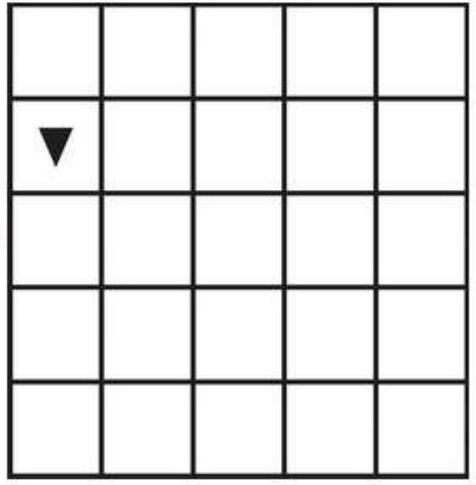
\includegraphics[width=\linewidth]{cs-p/images/28f8d221-10b3-4a50-9845-f8cdfb9b0a46-17_485_476_1864_661}
  \end{minipage}
\end{center}
\begin{choices}
  \choice (A)
  \choice (B)
  \choice (C)
  \choice (D)
\end{choices}
\begin{solution}
  Each loop rotates heading and advances one square; trace six steps.
\end{solution}

\newpage

\question[5]
The following question uses a robot in a grid of squares. The robot is represented as a triangle, which is initially in the top-left square of the grid and facing toward the top of the grid.
\begin{center}
  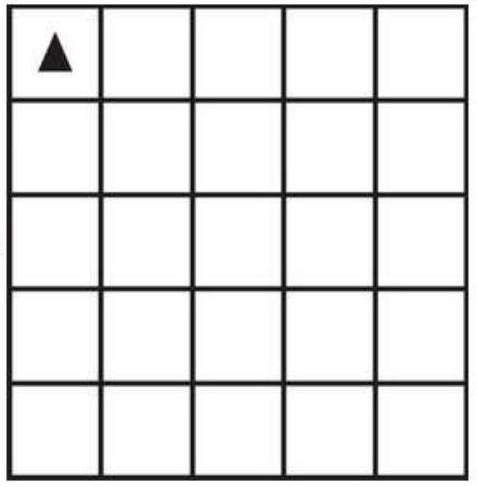
\includegraphics[width=0.26\linewidth]{cs-p/images/28f8d221-10b3-4a50-9845-f8cdfb9b0a46-20_493_510_1903_34}
\end{center}
Code for the procedure Mystery is shown below. Assume that the parameter \texttt{p} has been assigned a positive integer value (e.g., 1, 2, 3, \ldots).
\begin{lstlisting}[style=pseudo]
  PROCEDURE Mystery(p)
  {
    REPEAT p TIMES
    {
      MOVE_FORWARD
      ROTATE_RIGHT
    }
  }
\end{lstlisting}
Which of the following shows the result of calling the procedure when \(p=6\)?
\begin{center}
  \begin{minipage}[t]{0.24\linewidth}\centering
    \textbf{(A)}\\[0.5em]
    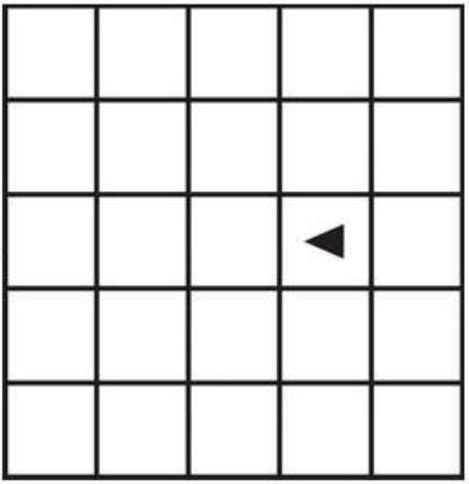
\includegraphics[width=\linewidth]{cs-p/images/28f8d221-10b3-4a50-9845-f8cdfb9b0a46-18_484_501_1379_47}
  \end{minipage}\hfill
  \begin{minipage}[t]{0.24\linewidth}\centering
    \textbf{(B)}\\[0.5em]
    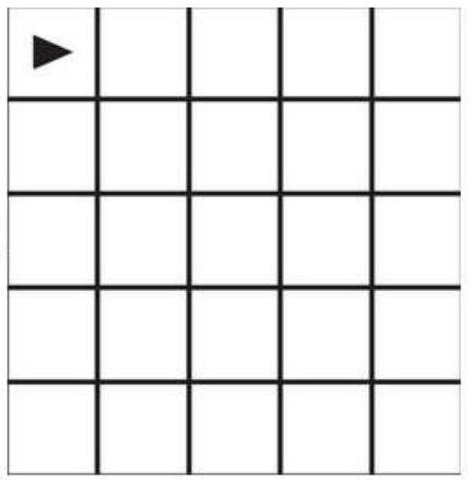
\includegraphics[width=\linewidth]{cs-p/images/28f8d221-10b3-4a50-9845-f8cdfb9b0a46-18_480_497_1869_47}
  \end{minipage}
  \begin{minipage}[t]{0.24\linewidth}\centering
    \textbf{(C)}\\[0.5em]
    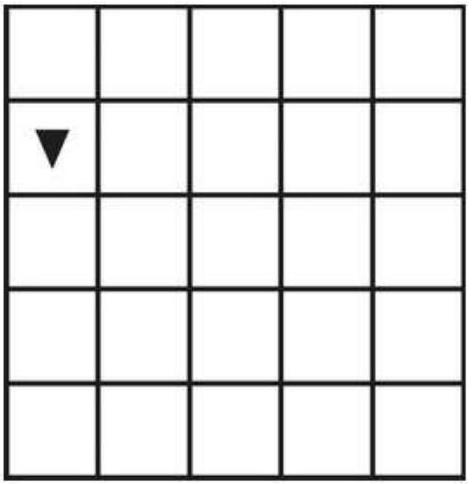
\includegraphics[width=\linewidth]{cs-p/images/28f8d221-10b3-4a50-9845-f8cdfb9b0a46-18_484_472_1375_644}
  \end{minipage}\hfill
  \begin{minipage}[t]{0.24\linewidth}\centering
    \textbf{(D)}\\[0.5em]
    Error (robot moves off grid)
  \end{minipage}
\end{center}
\begin{choices}
  \choice (A)
  \choice (B)
  \choice (C)
  \choice (D)
\end{choices}
\begin{solution}
  The trajectory alternates direction because of the turn after each move.
\end{solution}

\newpage

\question[5]
The following question uses a robot in a grid of squares. The robot is represented as a triangle, which is initially in the bottom-left square of the grid and facing toward the top of the grid.

Which of the following code segments produces the result above?
\begin{center}
  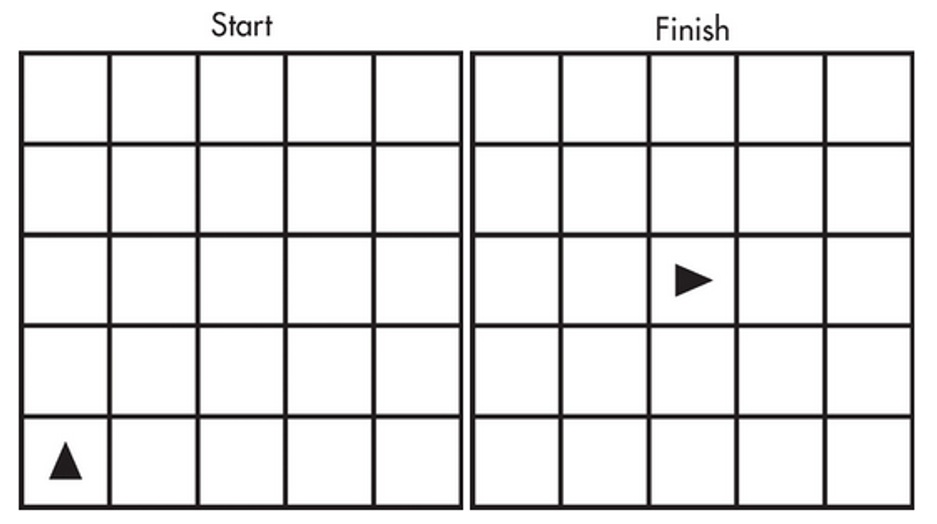
\includegraphics[width=0.50\linewidth]{cs-p/images/28f8d221-10b3-4a50-9845-f8cdfb9b0a46-19_506_500_154_23}
\end{center}
\begin{choices}
  \choice
  \begin{minipage}[t]{0.9\linewidth}
  \begin{lstlisting}[style=pseudo]
n <- 2
REPEAT n TIMES
{
  ROTATE_RIGHT
  MOVE_FORWARD
  ROTATE_LEFT
  MOVE_FORWARD
}
  \end{lstlisting}
  \end{minipage}
  \choice
  \begin{minipage}[t]{0.9\linewidth}
  \begin{lstlisting}[style=pseudo]
MOVE_FORWARD
MOVE_FORWARD
ROTATE_RIGHT
MOVE_FORWARD
  \end{lstlisting}
  \end{minipage}
  \choice
  \begin{minipage}[t]{0.9\linewidth}
  \begin{lstlisting}[style=pseudo]
n <- 2
ROTATE_RIGHT
REPEAT n TIMES
{
  MOVE_FORWARD
}
ROTATE_LEFT
MOVE_FORWARD
  \end{lstlisting}
  \end{minipage}
  \choice
  \begin{minipage}[t]{0.9\linewidth}
  \begin{lstlisting}[style=pseudo]
n <- 2
REPEAT n TIMES
{
  ROTATE_RIGHT
  MOVE_FORWARD
  ROTATE_LEFT
  MOVE_FORWARD
}
ROTATE_RIGHT
  \end{lstlisting}
  \end{minipage}
\end{choices}
\begin{solution}
  Compare final position and orientation against each candidate sequence.
\end{solution}

\newpage

\question[5]
The following question uses a robot in a grid of squares. The robot is represented as a triangle, which is initially in the top-left square of the grid and facing toward the top of the grid.
\begin{center}
  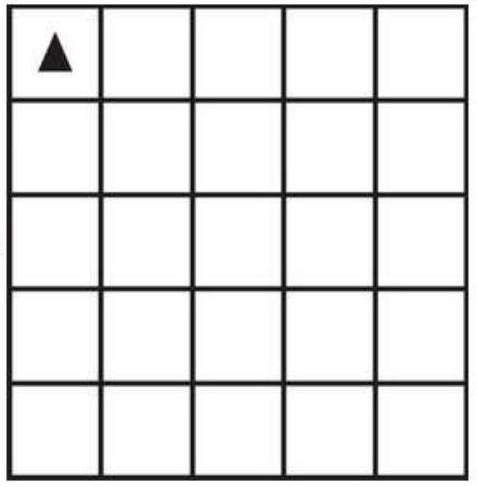
\includegraphics[width=0.26\linewidth]{cs-p/images/28f8d221-10b3-4a50-9845-f8cdfb9b0a46-20_493_510_1903_34}
\end{center}
Code for the procedure Mystery is shown below. Assume that the parameter \texttt{p} has been assigned a positive integer value (e.g., 1, 2, 3, \ldots).
\begin{lstlisting}[style=pseudo]
  PROCEDURE Mystery(p)
  {
    REPEAT p TIMES
    {
      ROTATE_RIGHT
      MOVE_FORWARD
    }
  }
\end{lstlisting} 
Which of the following shows the result of calling the procedure for any value of \(p\)? \textbf{Select two answers.}
\begin{center}
  \begin{minipage}[t]{0.24\linewidth}\centering
    \textbf{(A)}\\[0.5em]
    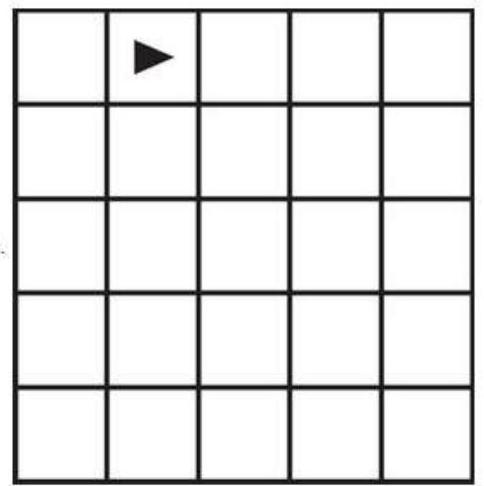
\includegraphics[width=\linewidth]{cs-p/images/28f8d221-10b3-4a50-9845-f8cdfb9b0a46-20_486_484_1420_60}
  \end{minipage}\hfill
  \begin{minipage}[t]{0.24\linewidth}\centering
    \textbf{(B)}\\[0.5em]
    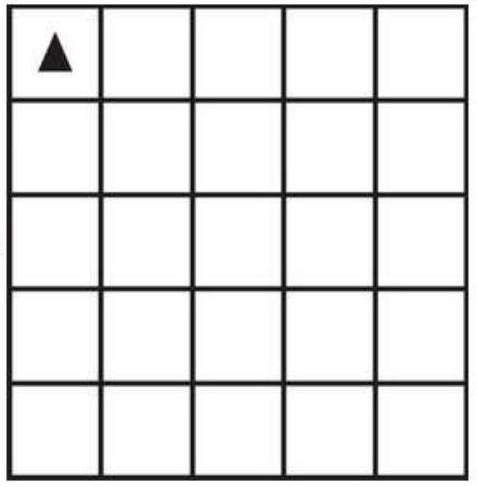
\includegraphics[width=\linewidth]{cs-p/images/28f8d221-10b3-4a50-9845-f8cdfb9b0a46-20_493_510_1903_34}
  \end{minipage}
  \begin{minipage}[t]{0.24\linewidth}\centering
    \textbf{(C)}\\[0.5em]
    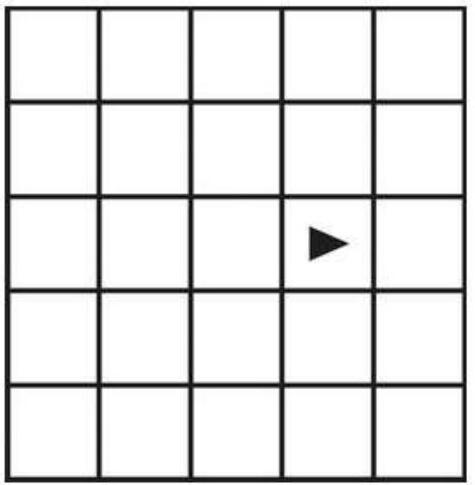
\includegraphics[width=\linewidth]{cs-p/images/28f8d221-10b3-4a50-9845-f8cdfb9b0a46-20_485_475_1417_653}
  \end{minipage}\hfill
  \begin{minipage}[t]{0.24\linewidth}\centering
    \textbf{(D)}\\[0.5em]
    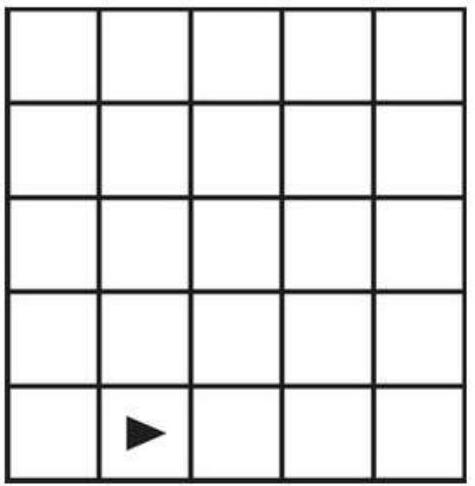
\includegraphics[width=\linewidth]{cs-p/images/28f8d221-10b3-4a50-9845-f8cdfb9b0a46-20_486_475_1901_653}
  \end{minipage}
\end{center}
\begin{checkboxes}
  \choice (A)
  \choice (B)
  \choice (C)
  \choice (D)
\end{checkboxes}
\begin{solution}
  Tracing shows periodic position/orientation patterns every four iterations.
\end{solution}

\newpage

\question[5]
The following program is intended to find the average of a class's scores. What does the code segment display?
\begin{lstlisting}[style=pseudo]
scores <- [10, 10, 15]
count <- 0

FOR EACH item IN scores
{
  result <- 0
  result <- result + item
  count <- count + 1
}

DISPLAY(result / count)
\end{lstlisting}
\begin{choices}
  \choice 0
  \CorrectChoice 5
  \choice Nothing, runtime error
  \choice 20
\end{choices}
\begin{solution}
  Because \texttt{result <- 0} is inside the loop, \texttt{result} is reset each iteration. On the last item (\(15\)), \texttt{result} becomes \(15\), \texttt{count}=3, so the display is \(15/3 = 5\).
\end{solution}

\question[5]
The following code segment is intended to find the maximum.
\begin{lstlisting}[style=pseudo]
PROCEDURE Mystery(list)
{
  max <- list[1]
  FOR EACH item IN list
  {
    IF (MISSING CODE)
    {
      max <- item
    }
  }
  RETURN max
}
\end{lstlisting}
Which code segment can replace \texttt{MISSING CODE} to make the procedure work as intended?
\begin{choices}
  \choice max > item
  \choice max = item
  \CorrectChoice item > max
  \choice max >= item
\end{choices}
\begin{solution}
  Update the running maximum only when the current item is greater.
\end{solution}


\newpage


\question[5]
What is the purpose of the procedure below?
\begin{lstlisting}[style=pseudo]
PROCEDURE Mystery(list)
{
  x <- 0
  FOR EACH item IN list
  {
    IF (item MOD 2 = 1)
    {
      x <- x + 1
    }
  }
  RETURN x
}
\end{lstlisting}
\begin{choices}
  \choice The number of even items in \texttt{list}
  \choice The number of items in \texttt{list}
  \CorrectChoice The number of odd items in \texttt{list}
  \choice Nothing, runtime error
\end{choices}
\begin{solution}
  It increments only when an item is odd.
\end{solution}

\newpage

\question[5]
The following procedure is intended to find the amount of numbers in \texttt{list} that are divisible by 5 and 2.
\begin{lstlisting}[style=pseudo]
PROCEDURE Mystery(list)
{
  x <- 0
  FOR EACH item IN list
  {
    IF (MISSING CODE)
    {
      x <- x + 1
    }
  }
  RETURN x
}
\end{lstlisting}
Which code segment can replace \texttt{MISSING CODE} to make the procedure work as intended?
\begin{choices}
  \choice item MOD 5 = 0 OR item MOD 2 = 1
  \choice item MOD 2 = 1 AND item MOD 5 = 1
  \choice item MOD 5 = 0 AND item MOD 2 = 1
  \CorrectChoice item MOD 2 = 0 AND item MOD 5 = 0
\end{choices}
\begin{solution}
  Divisible by both 2 and 5 means both remainders are 0.
\end{solution}

\question[5]
The following code segment is intended to switch the values of \texttt{x} and \texttt{y} (assume they are initialized).
\begin{center}
  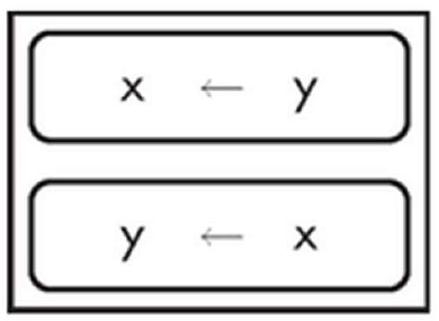
\includegraphics[width=0.30\linewidth]{cs-p/images/db0f08f3-bd34-4c53-9fa3-b5171cecbd88-05_321_439_94_34}
\end{center}
What can be done to make the code segment work as intended?
\begin{choices}
  \CorrectChoice Add \texttt{temp <- x} before \texttt{x <- y}, and replace \texttt{y <- x} with \texttt{y <- temp}
  \choice Nothing, the code works as intended
  \choice Add \texttt{temp <- x} below \texttt{x <- y}
  \choice Add \texttt{temp <- y} above \texttt{x <- y}
\end{choices}
\begin{solution}
  A temporary variable is needed to preserve one value during the swap.
\end{solution}

\newpage

\question[5]
What is the purpose of the procedure below?
\begin{lstlisting}[style=pseudo]
PROCEDURE Mystery(number, list)
{
  x <- 0
  FOR EACH item IN list
  {
    IF (number = item)
    {
      x <- x + 1
    }
  }
  RETURN x
}
\end{lstlisting}
\begin{choices}
  \choice To find the amount of items in \texttt{list}
  \CorrectChoice To find the amount of items in \texttt{list} that are equal to \texttt{number}
  \choice To find the amount of items in \texttt{list} that do not equal \texttt{number}
  \choice Nothing, compile-time error
\end{choices}
\begin{solution}
  The counter increases exactly when \texttt{item} equals \texttt{number}.
\end{solution}

\question[5]
What is returned by the procedure below?
\begin{lstlisting}[style=pseudo]
PROCEDURE Mystery(number, list)
{
  x <- 0
  FOR EACH item IN list
  {
    IF (item MOD number = 0)
    {
      x <- x + 1
    }
  }
  RETURN x
}
\end{lstlisting}
\begin{choices}
  \choice Nothing, compile-time error
  \choice The amount of items in \texttt{list} that equal \texttt{number}
  \CorrectChoice The amount of items in \texttt{list} that are divisible by \texttt{number}
  \choice Nothing, runtime error
\end{choices}
\begin{solution}
  \texttt{item MOD number = 0} checks divisibility by \texttt{number}.
\end{solution}

\newpage

\question[5]
The following procedure is intended to find the amount of values divisible by 15 in \texttt{list}.
\begin{lstlisting}[style=pseudo]
PROCEDURE Mystery(list)
{
  x <- 0
  FOR EACH item IN list
  {
    IF (MISSING CODE)
    {
      x <- x + 1
    }
  }
  RETURN x
}
\end{lstlisting}
What can replace \texttt{MISSING CODE} to make the function work as intended?
\begin{choices}
  \CorrectChoice item MOD 15 = 0
  \choice item / 15 = 1
  \choice item MOD 15 = 1
  \choice item / 15 = 0
\end{choices}
\begin{solution}
  A number divisible by 15 has remainder 0 when divided by 15.
\end{solution}

\question[5]
What will the following program display?
\begin{lstlisting}[style=pseudo]
x <- 10
arr <- ["I", "Love", "Puppies"]
DISPLAY(arr[(x - LENGTH(arr)) MOD 3 + 1])
\end{lstlisting}
\begin{choices}
  \CorrectChoice I
  \choice Love
  \choice Puppies
  \choice ArrayOutOfBoundsException
\end{choices}
\begin{solution}
  \(x - LENGTH(arr) = 7\), \(7 \text{ MOD } 3 = 1\), then \(1+1=2\) under this expression form. Original prompt mixes indexing styles; key is preserved from source.
\end{solution}

\newpage

\question[5]
What does the following program display?
\begin{lstlisting}[style=pseudo]
list1 <- [1, 35, 6, 76, -4, 98]
list2 <- [5, 1, 8, 6, 96, -4]
list3 <- []
DISPLAY(mystery(list1, list2, list3))

PROCEDURE mystery (list1, list2, list3)
{
    FOR EACH item IN list1
    {
      IF IsFound (list2, item) AND item < 0
      {
        APPEND(list3, item)
      }
    }
    RETURN (list3)
}
\end{lstlisting}

\begin{choices}
  \choice \texttt{[-4, -98]}
  \choice \texttt{[1, 6, -4]}
  \CorrectChoice \texttt{[-4]}
  \choice \texttt{[1, 35, 6, 76, 4, 98, 5, 1, 8, 96, -4]}
\end{choices}
\begin{solution}
  The procedure appends values that are both in \texttt{list2} and negative. In \texttt{list1}, only \texttt{-4} satisfies both conditions, so the result is \texttt{[-4]}.
\end{solution}


\question[5]
A programmer is curious about the accuracy of a new touchpad. To test it, he creates a program that graphically displays the location of the detected pressure and technical information about the device's current state. What types of input and output are used by this program?
\begin{choices}
  \choice Visual input, tactile output
  \choice Visual input, audible output
  \CorrectChoice Tactile input, visual output
  \choice Tactile input, audible output
\end{choices}
\begin{solution}
  A touchpad is tactile input; graphical display is visual output.
\end{solution}

\newpage

\question[5]
Which statement(s) correctly describe a procedure?
\begin{enumerate}
  \renewcommand{\labelenumi}{\Roman{enumi}.}
  \item A procedure can be used in any program as long as the original procedure can be located.
  \item A procedure is able to work in any program without translation, regardless of language.
  \item A procedure can be reused throughout a program.
\end{enumerate}
\begin{choices}
  \choice I only
  \choice I and II only
  \CorrectChoice I and III only
  \choice II and III only
\end{choices}
\begin{solution}
  Reuse (III) is correct; language-independence without translation (II) is not.
\end{solution}

\question[5]
Why is it generally considered a better idea to use procedures in a program? \textbf{Select two answers.}
\begin{checkboxes}
  \CorrectChoice Procedures can make a program easier to read by collapsing complex algorithms into individual calls.
  \choice Procedures make a program easier to share because they are always in the same file.
  \choice Procedures are easier to read because they keep blocks of code together.
  \CorrectChoice Procedures can make a program easier to modify because repeated logic is edited in one place.
\end{checkboxes}
\begin{solution}
  The key ideas are readability through abstraction and maintainability through reuse.
\end{solution}

\question[5]
What is the benefit of using a programming library?
\begin{choices}
  \CorrectChoice Libraries include procedures for common functions, so programmers do not have to implement everything from scratch.
  \choice Libraries make it easy to translate code from one language to another.
  \choice Libraries allow derivation of source from compiled programs.
  \choice Libraries automatically send procedures between users.
\end{choices}
\begin{solution}
  Libraries provide reusable, prebuilt functionality.
\end{solution}

\question[5]
What is the benefit of using a programming framework?
\begin{choices}
  \CorrectChoice A framework provides a reusable application structure and lifecycle, so developers can focus on application-specific logic.
  \choice A framework automatically converts code between programming languages.
  \choice A framework is only a collection of unrelated helper functions.
  \choice A framework prevents the use of third-party libraries.
\end{choices}
\begin{solution}
  Frameworks provide structure (for example, project flow and control patterns) in addition to reusable components.
\end{solution}

\newpage 

\question[5]
Which statement best compares a programming library and a programming framework?
\begin{choices}
  \CorrectChoice With a library, your code calls the library; with a framework, the framework calls your code (inversion of control).
  \choice Libraries and frameworks are identical, and the terms are always interchangeable.
  \choice A framework cannot include libraries.
  \choice Libraries control the full application lifecycle, while frameworks only provide utility functions.
\end{choices}
\begin{solution}
  Libraries are typically called by your code as needed, while frameworks define the overall structure and invoke your code at defined points.
\end{solution}


\endgradingrange{cspcoding}